\section{Повышение точности обработки температурных кинетик в методе	пьезоэлектрической резонансной калориметрии}

\begin{frame}
	\frametitle{3. Повышение точности обработки температурных кинетик в методе ПРЛК}
	
	\begin{center}
		\centering
		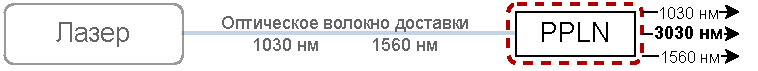
\includegraphics[width=0.67\linewidth]{Presentation/images/problem_ppln}
	\end{center}
	
%	\fixme{Актуальность: мало 3 мкм <- нарушение условий фазового синхронизма <- разогрев кристалла <- оптическое поглощение <- необходимость его точного определения}
	
%	Метод~--- лазерная калориметрия\footnote{ГОСТ Р ИСО 11551-2015. Методика измерений коэффициента поглощения лазерного излучения оптическими элементами. Введ. 07.08.2015. М: Стандартинформ, 2017. 20 с.}:
	\vspace{-0.2cm}
	
	\begin{columns}[t]
		\begin{column}{0.47\textwidth}	
			\small		
			Лазерная калориметрия (ЛК):
			
			\begin{center}
				\centering
				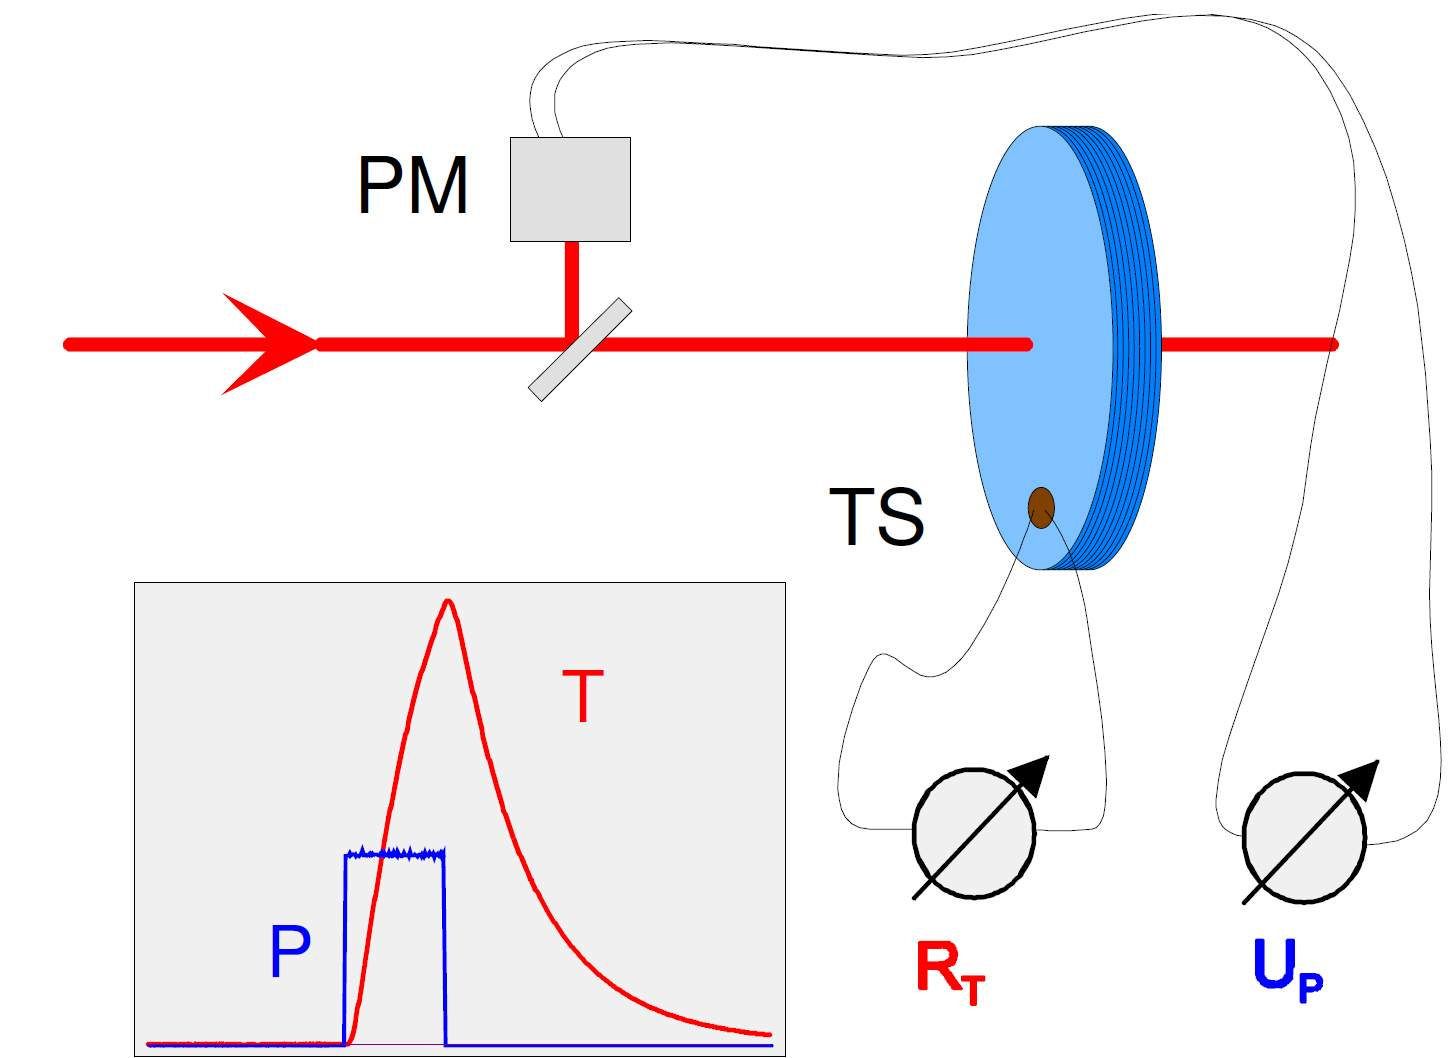
\includegraphics[height=1.75cm]{Presentation/images/lk}
			\end{center}
			
			\vspace{-0.5cm}
			
			\begin{itemize}
				\setlength{\itemsep}{0.5em}
				\item Нагрев образца излучением $P$, температура $T$: внешний термодатчик TS
				\item Ограничения: теплопроводность образца, рассеянное излучение, тепловой контакт
			\end{itemize}

			
		\end{column}
		\begin{column}{0.53\textwidth}
			\small
			Пьезоэлектрическая резонансная ЛК (ПРЛК):
			
			\begin{center}
				\centering
				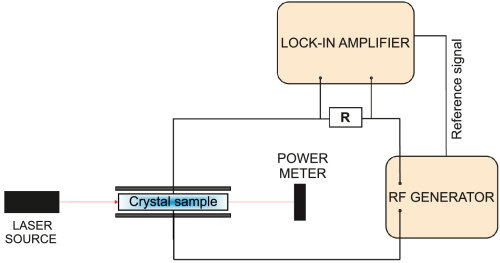
\includegraphics[height=1.74cm]{Presentation/images/prlc}
			\end{center}
			
			\vspace{-0.5cm}
			
			\begin{itemize}
				\setlength{\itemsep}{0.3em}
				\item Акустические моды н-о кристаллов возбуждаются внешним РЧ полем (обратный пьезоэффект)
				
				\item $T$ определяется по сдвигу частоты мод
				
				\item После калибровки сдвиг пересчитывается в $T$
				
				\item Даёт среднюю температуру кристалла\footnotemark
			\end{itemize}
		\end{column}
	\end{columns}	
	\footnotetext{\scriptsize G. Aloyan, N. Kovalenko, I. Grishchenko, A. Konyashkin, and O. Ryabushkin, “Acoustic resonance spectroscopy of piezoelectric crystals under non-uniform heating,” Acoustical Physics, vol. 68, no. 5, pp. 427–434, 2022}
\end{frame}


\begin{frame}
	\frametitle{3. Повышение точности обработки температурных кинетик в методе ПРЛК}
%	\framesubtitle{Пьезоэлектрическая резонансная лазерная калориметрия}
	
	Уравнение теплового баланса, приближение бесконечной теплопроводности:
	
	\vspace{0.3cm}
	
	\begin{columns}
		
		\begin{column}{0.5\textwidth}
			\[
			\begin{cases}
				\dfrac{d T}{d t} = \overline{Q}\theta(t_0 - t) - \Gamma(T - T_a) \\
				T(0) = T_a
			\end{cases}
			\]
			
			Решение:			
			\[
			T(t) = T_a + \frac{\overline{Q}}{\Gamma}
			\begin{cases}
				1 - e^{-\Gamma t}, & t \leq t_0, \\
				e^{-\Gamma t}(e^{\Gamma t_0} - 1), & t > t_0
			\end{cases}
			\]
			
			Аппроксимация:
			
			\[
				f(t) = A + Be^{-Ct}
			\]
			
		\end{column}'
		
		\begin{column}{0.5\textwidth}
			{\linespread{1.2}\selectfont\small{$\overline{Q} = \alpha LP/(mc_{\text{sp}})$ --- усреднённый по образцу тепловой источник, связанный с поглощением лазерного излучения при малом оптическом поглощении,
				
			$\alpha$~--- коэффициент поглощения,
			
			$L, m, c_{\text{sp}}$~--- длина, масса, удельная теплоёмкость кристалла,
			
			$P$ --- мощность излучения,
			
			$\Gamma = hS/(mc_{\text{sp}})$ --- скорость теплоотдачи,
			
			$h$ --- коэффициент теплоотдачи,
			
			$S$ --- площадь поверхности образца,
			
			$T_a$ --- температура окружающей среды,
			
			$t_0$ --- выключение лазера}}
		\end{column}
		
	\end{columns}	
\end{frame}


\begin{frame}
	\frametitle{3. Повышение точности обработки температурных кинетик в методе ПРЛК}	
	\vspace{-0.18cm}
	\begin{columns}
		\small
		\begin{column}{0.63\textwidth}	
			Методики обработки температурных кинетик\footnotemark:		
			\begin{itemize}
				\setlength{\itemsep}{-5pt}
				\item \textbf{Экспоненциальная}: аппроксимация кинетики разогрева \[E = -B_{\text{exp}}C_{\text{exp}} = \overline{Q};\]
				\item \textbf{Импульсная}: экстраполяция кинетики остывания \[I = \frac{C_{\text{puls}}f(t_0/2)}{2\sinh(C_{\text{puls}}t_0/2)} = \overline{Q};\]
				\item \textbf{Градиентная}: разность производных разогрева и остывания (исключена из стандарта в 2003 году): \[G = \dfrac{d T}{d t} \bigg|_{t < t_0, T = T_0} - \dfrac{d T}{d t} \bigg|_{t > t_0, T = T_0}= \overline{Q}.\]
			\end{itemize}					
		\end{column}
		\begin{column}{0.37\textwidth}
			\begin{center}
				\centering
				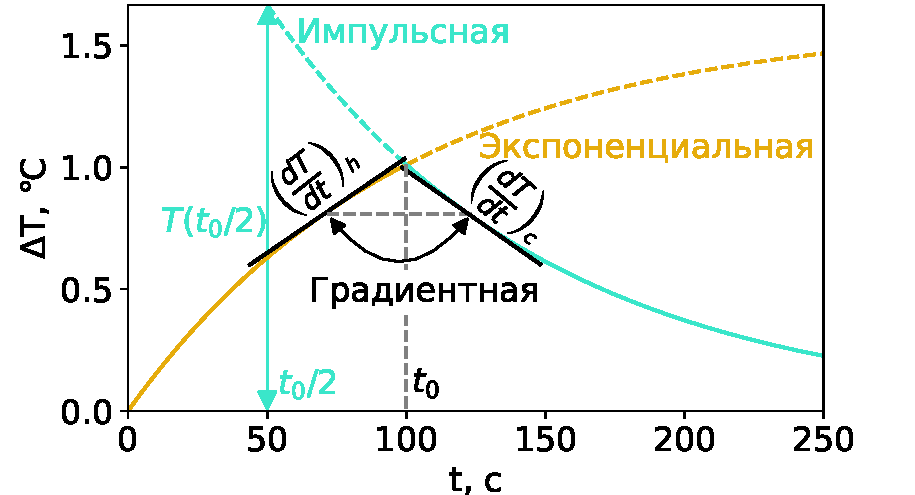
\includegraphics[width=\linewidth]{Presentation/images/illustrative_example}
				\footnotesize{Иллюстрация методик на примере кинетики нагрева и остывания}
			\end{center}
						
			\footnotesize{
					
			$B_{\text{exp}}$, $C_{\text{exp, puls}}$ --- параметры аппроксимации $f(t) = A + Be^{-Ct}$,
			
			$E, I, G$ --- величины тепловых источников по экспоненциальной, импульсной, градиентной методикам}
		\end{column}
	\end{columns}	
	\small
	В отсутствие погрешностей величина $\overline{Q}$ для трёх методик совпадает.
	\vfill
	
	\footnotetext{\tiny{ГОСТ Р ИСО 11551-2015 «Оптика и оптические приборы. Лазеры и лазерные установки (системы). Методика измерений коэффициента поглощения лазерного излучения оптическими элементами»}}
%	\footnotesize{$\alpha$~--- коэффициент поглощения, $L, m, c_{\text{sp}}$~--- длина, масса, удельная теплоёмкость кристалла, $P$ --- мощность излучения.}
\end{frame}

\begin{frame}
	\framesubtitle{Поправки к температурным кинетикам}
	\frametitle{Влияние непостоянства температуры окружающей среды}
	
	\centering
	Мотивация: суточный дрейф $T_a$, отсутствие термостатирования.\\Кинетика $T_a$ произвольная.
		
	\begin{columns}
		\begin{column}{0.55\textwidth}			
			\begin{itemize}
				\setlength{\itemsep}{13pt}
				\item \textbf{Экспоненциальная и импульсная} методики: корректировка кинетики перед аппроксимацией
				
				\( \epsilon(t) = \sum_{\omega_k} \dfrac{\im \omega_k \hat{T_a}(\omega_k)}{\Gamma + \im\omega_k} [\exp(-\Gamma t) - \exp(\im \omega_k t)] \)

				\item \textbf{Градиентная} методика: корректировка величины	 теплового источника
				
				\(
					G_{\text{corr}} \coloneqq G - \left(\dfrac{d T_a}{d t} \bigg|_{t < t_0, T = T_0} - \dfrac{d T_a}{ dt} \bigg|_{t > t_0, T = T_0}\right)
				\)
%				$\Gamma$ --- скорость теплоотдачи; $t$ --- время,	$t_0$ --- выключение лазера; $T_0$ --- фикс. температура.
			\end{itemize}			
			\vfill
			{\footnotesize $\epsilon$ --- поправка к $T(t)$;\\$\omega_k,\hat T_a(\omega_k)$ --- гармоники $T_a(t)$;}
		\end{column}
		\begin{column}{0.44\textwidth}
			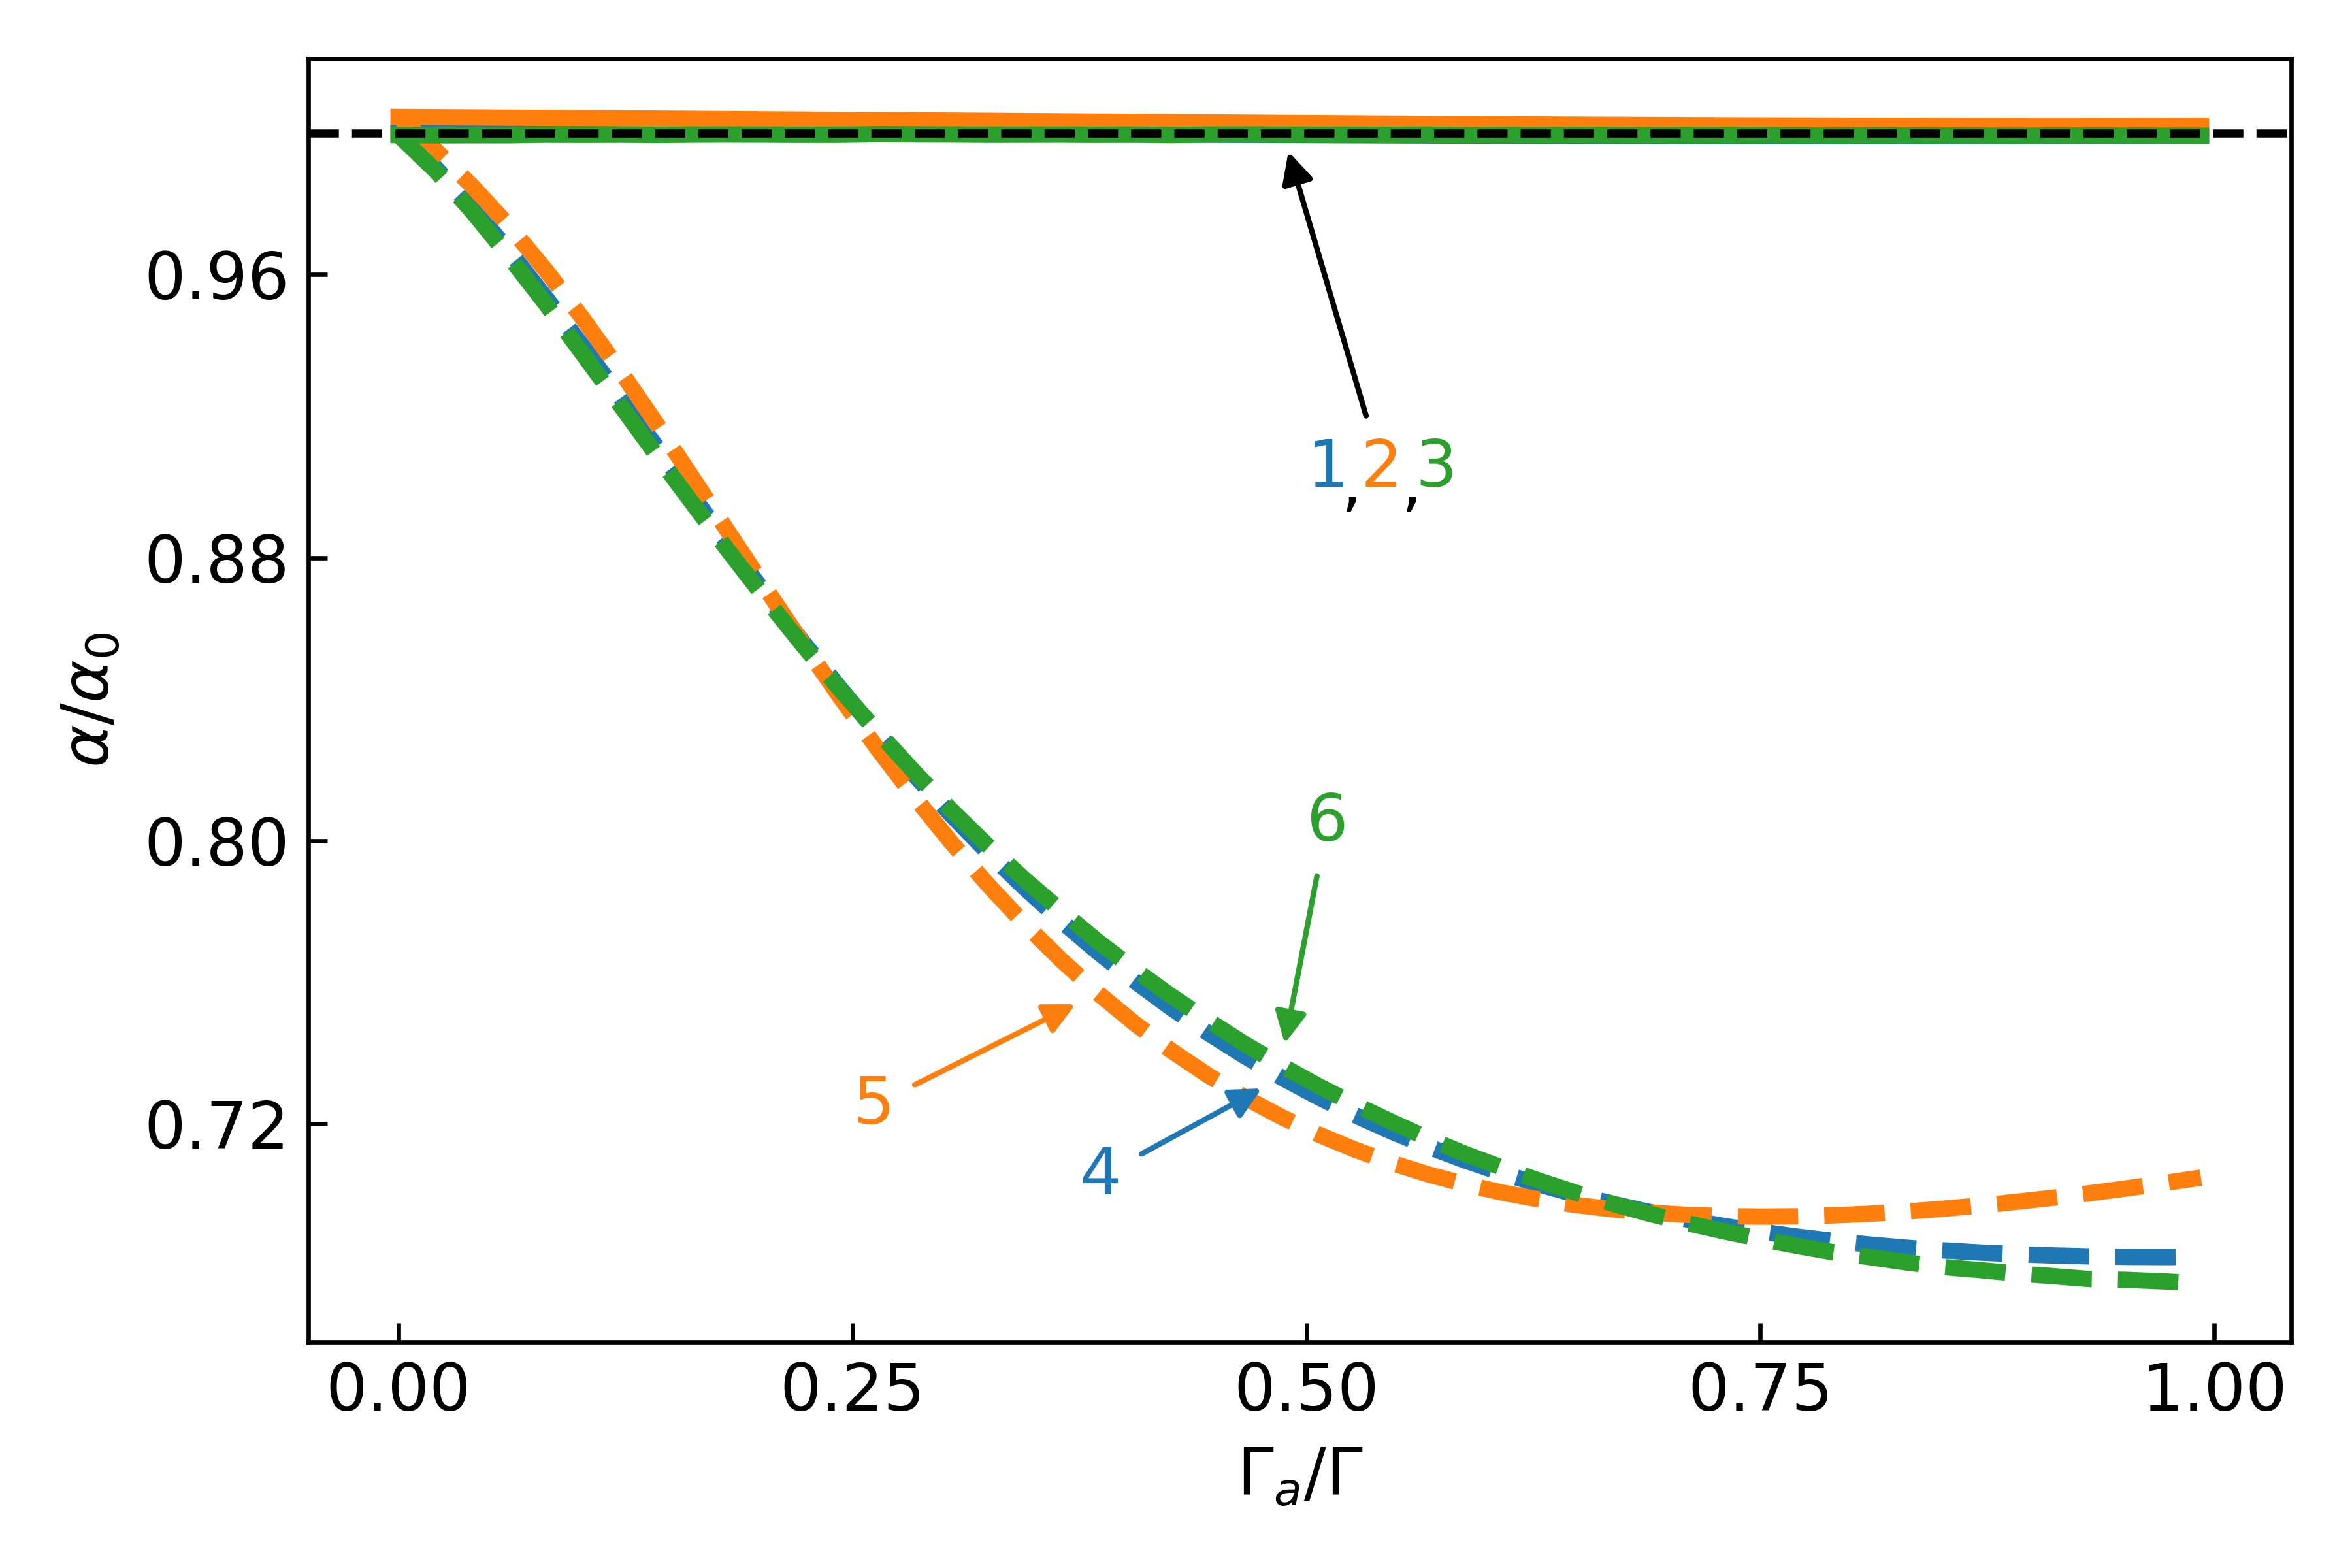
\includegraphics[width=\linewidth]{Dissertation/images/gradient/fourier_ambient_exp}
			\centering
			\footnotesize{Зависимость погрешности определения коэффициента поглощения $\alpha/\alpha_0$ от отношения скоростей теплоотдачи окружающей среды и кристалла $\Gamma_a/\Gamma$.\\1--3: {\color{defcolor1}{экспоненциальная}}, {\color{defcolor2}{импульсная}}, {\color{defcolor3}{градиентная}} с учётом поправки;\\4--6: без коррекции}
		\end{column}
	\end{columns}	
\end{frame}


\begin{frame}
	\framesubtitle{Поправки к температурным кинетикам}
	\frametitle{Влияние непостоянства коэффициента теплоотдачи}
	
	\begin{columns}
		\small
		\begin{column}{0.7\textwidth}			
			Мотивация: неконтролируемый теплообмен. Пусть различные, но постоянные $h$ при нагреве и охлаждении.			
		\end{column}
		\begin{column}{0.3\textwidth}
			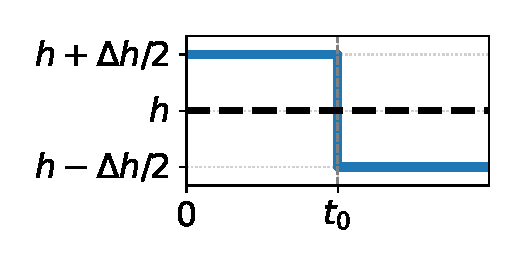
\includegraphics[height=1.7cm]{Presentation/images/h_vs_t}
		\end{column}
	\end{columns}	
	
	\vspace{-0.2cm}
	
	\begin{columns}
		\small
		\begin{column}{0.55\textwidth}			
			\begin{itemize}
				\setlength{\itemsep}{10pt}
				\item \textbf{Экспоненциальная}: без изменений	
				\item \textbf{Импульсная}: 
								
				\begin{equation*}
					I_{\text{corr}} := \frac{C_{\mathrm{exp}} f_{\mathrm{puls}}\left( {t_0}/2 \right)}
					{\exp \left( C_{\mathrm{puls}} {t_0}/{2} \right) - \exp \left( -C_{\mathrm{exp}} {t_0}/{2} \right)}
				\end{equation*}
				
				\item \textbf{Градиентная}: 
				
				\begin{equation*}
					G_{\text{corr}} \coloneqq G + {T_0}\left( {{C_{\text{exp}}} - {C_{\text{puls}}}} \right)
				\end{equation*}
				
				\footnotesize{$f_{\mathrm{puls}}$ --- экстраполяция кинетики остывания;\\ $C_{\mathrm{exp}},C_{\mathrm{puls}}$ --- показатели экспонент нагрева/остывания}
			\end{itemize}			
		\end{column}
		\begin{column}{0.44\textwidth}
			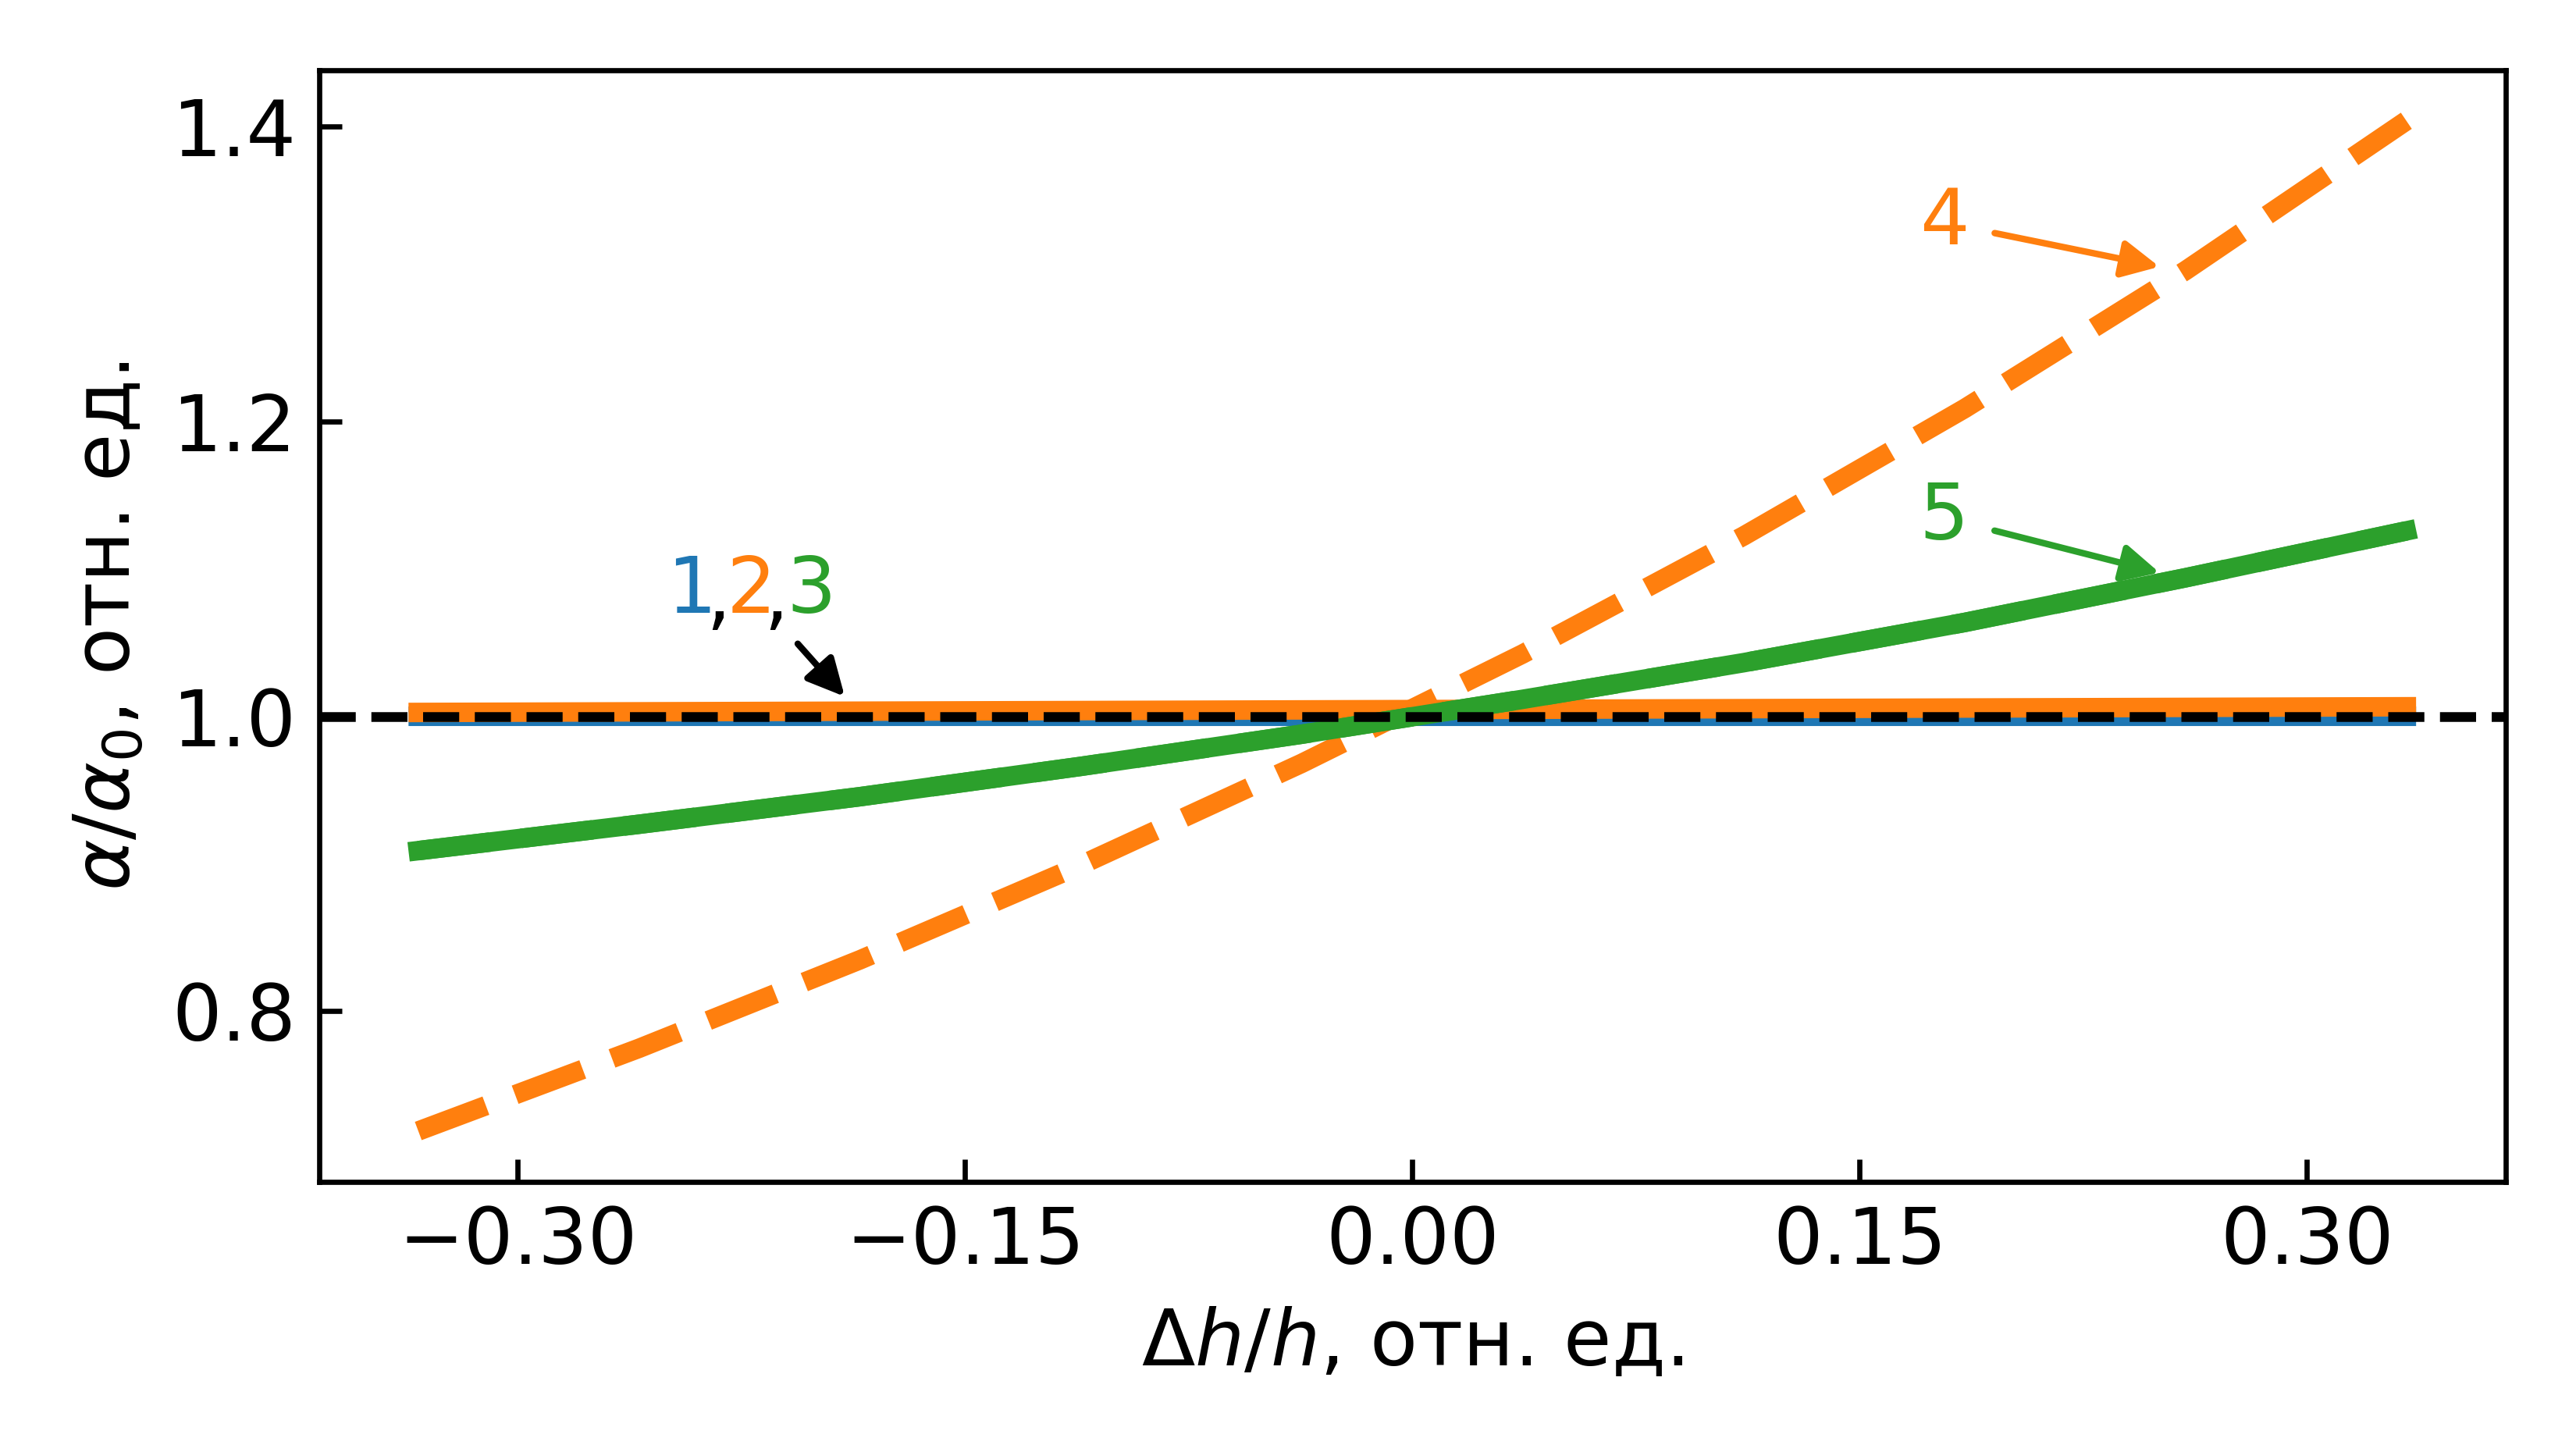
\includegraphics[width=\linewidth]{Dissertation/images/gradient/heat_transfer_account_var3}
			\centering
			\footnotesize{Зависимость $\alpha/\alpha_0$ от относительного изменения коэффициента теплоотдачи $\Delta h / h$.\\1~--- {\color{defcolor1}{экспоненциальная}},\\2,~3~--- {\color{defcolor2}{импульсная}}, {\color{defcolor3}{градиентная}} с коррекцией;\\4,~5--- {\color{defcolor2}{импульсная}}, {\color{defcolor3}{градиентная}} без коррекции}
		\end{column}
	\end{columns}	
\end{frame}

\begin{frame}
	\frametitle{Поправки к температурным кинетикам}
	\framesubtitle{Эксперимент}
	\begin{columns}		
		\begin{column}{0.28\textwidth}
			\raggedright
			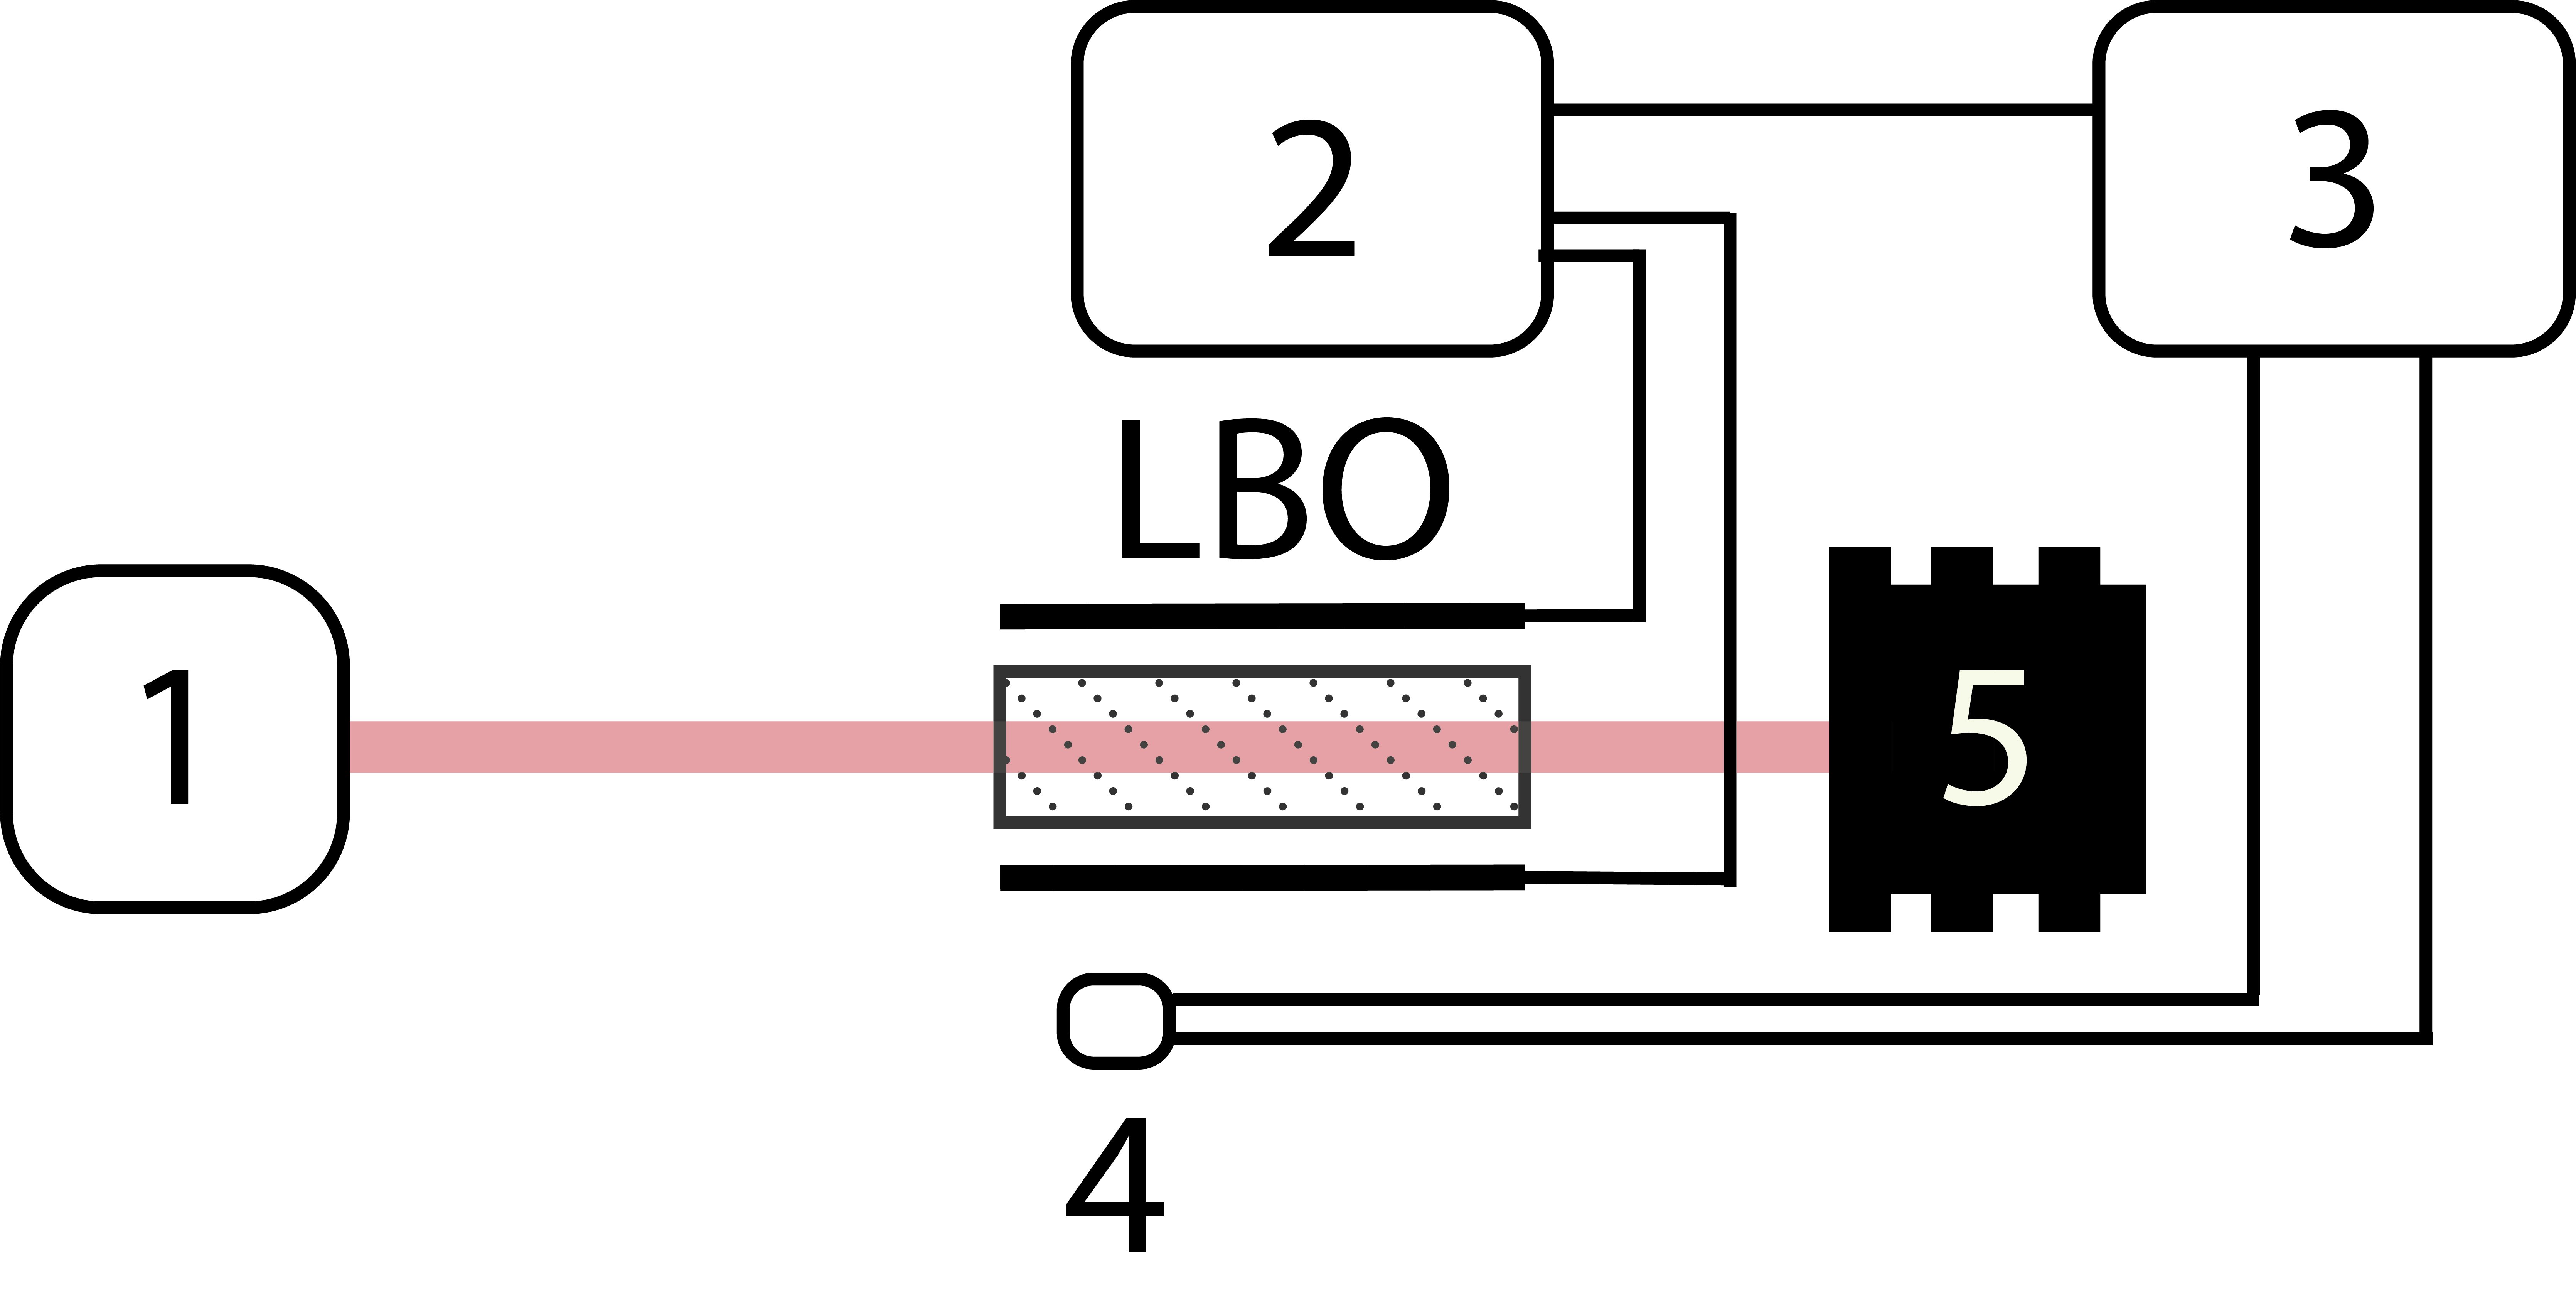
\includegraphics[width=0.99\linewidth]{Dissertation/images/gradient/scheme}	
			{\scriptsize}
		\end{column}

		\begin{column}{0.36\textwidth}
			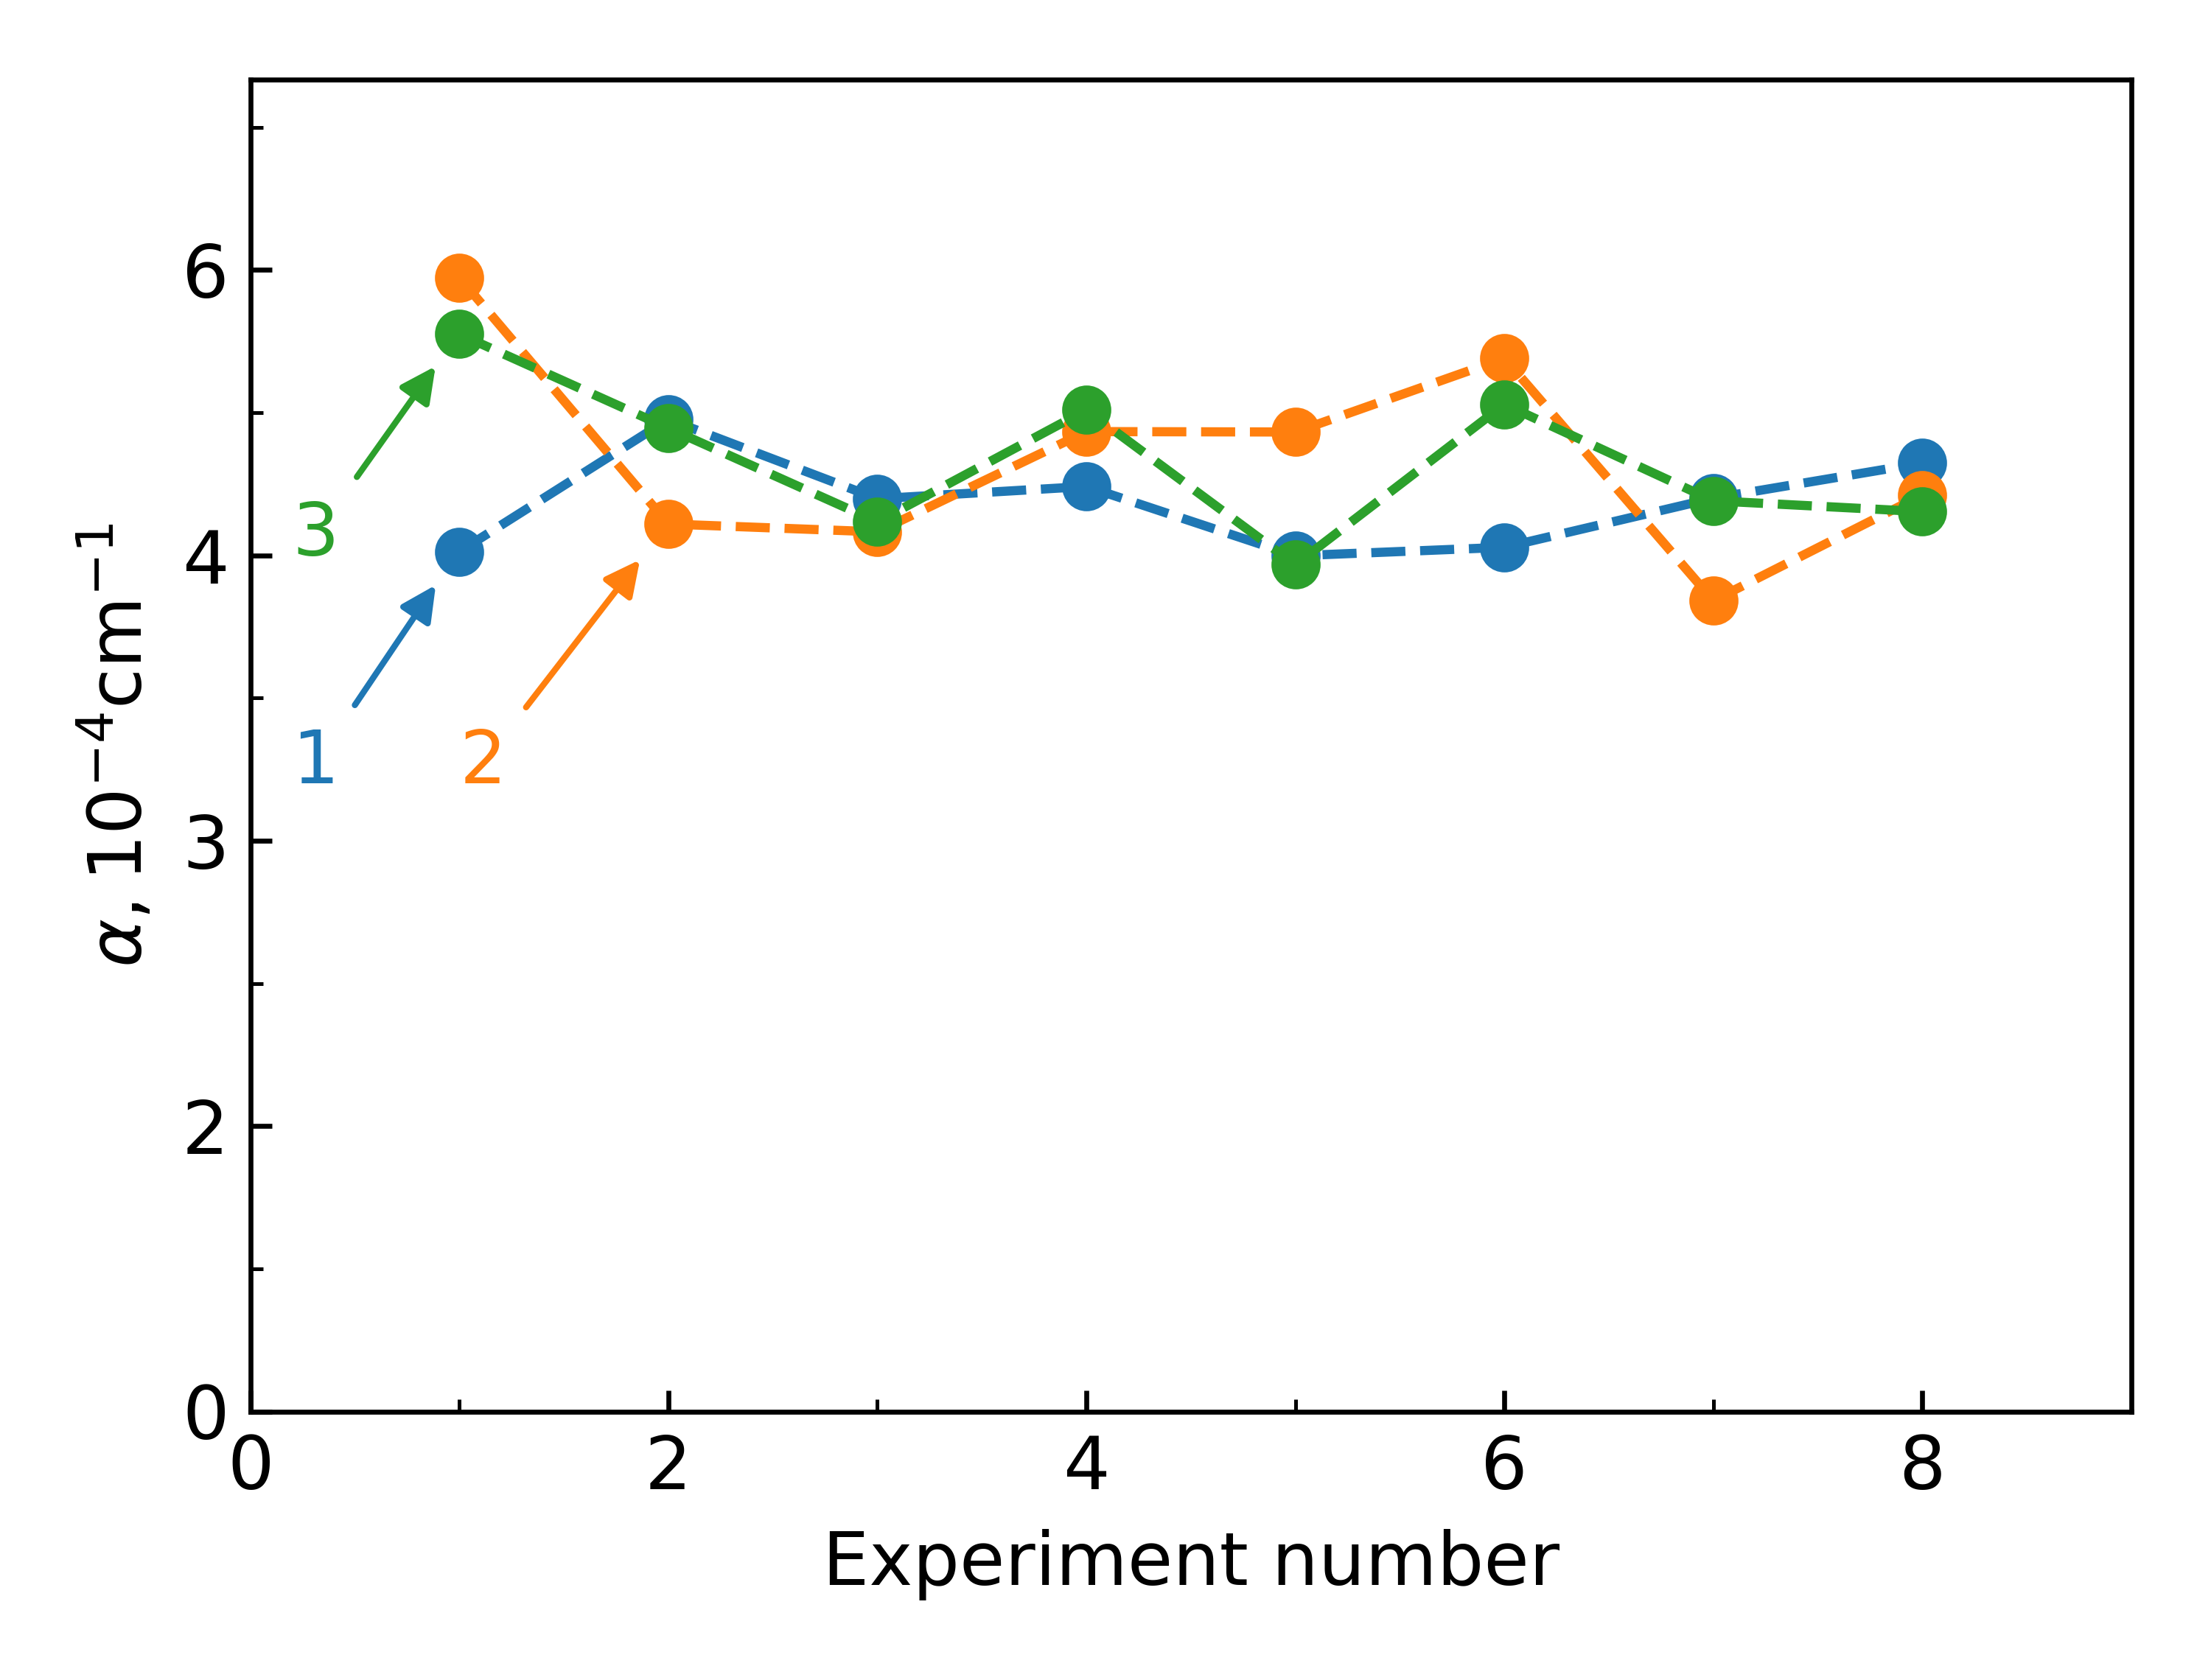
\includegraphics[width=\linewidth]{Dissertation/images/gradient/main_no_ambient_sub}
		\end{column}
		
		\begin{column}{0.36\textwidth}
			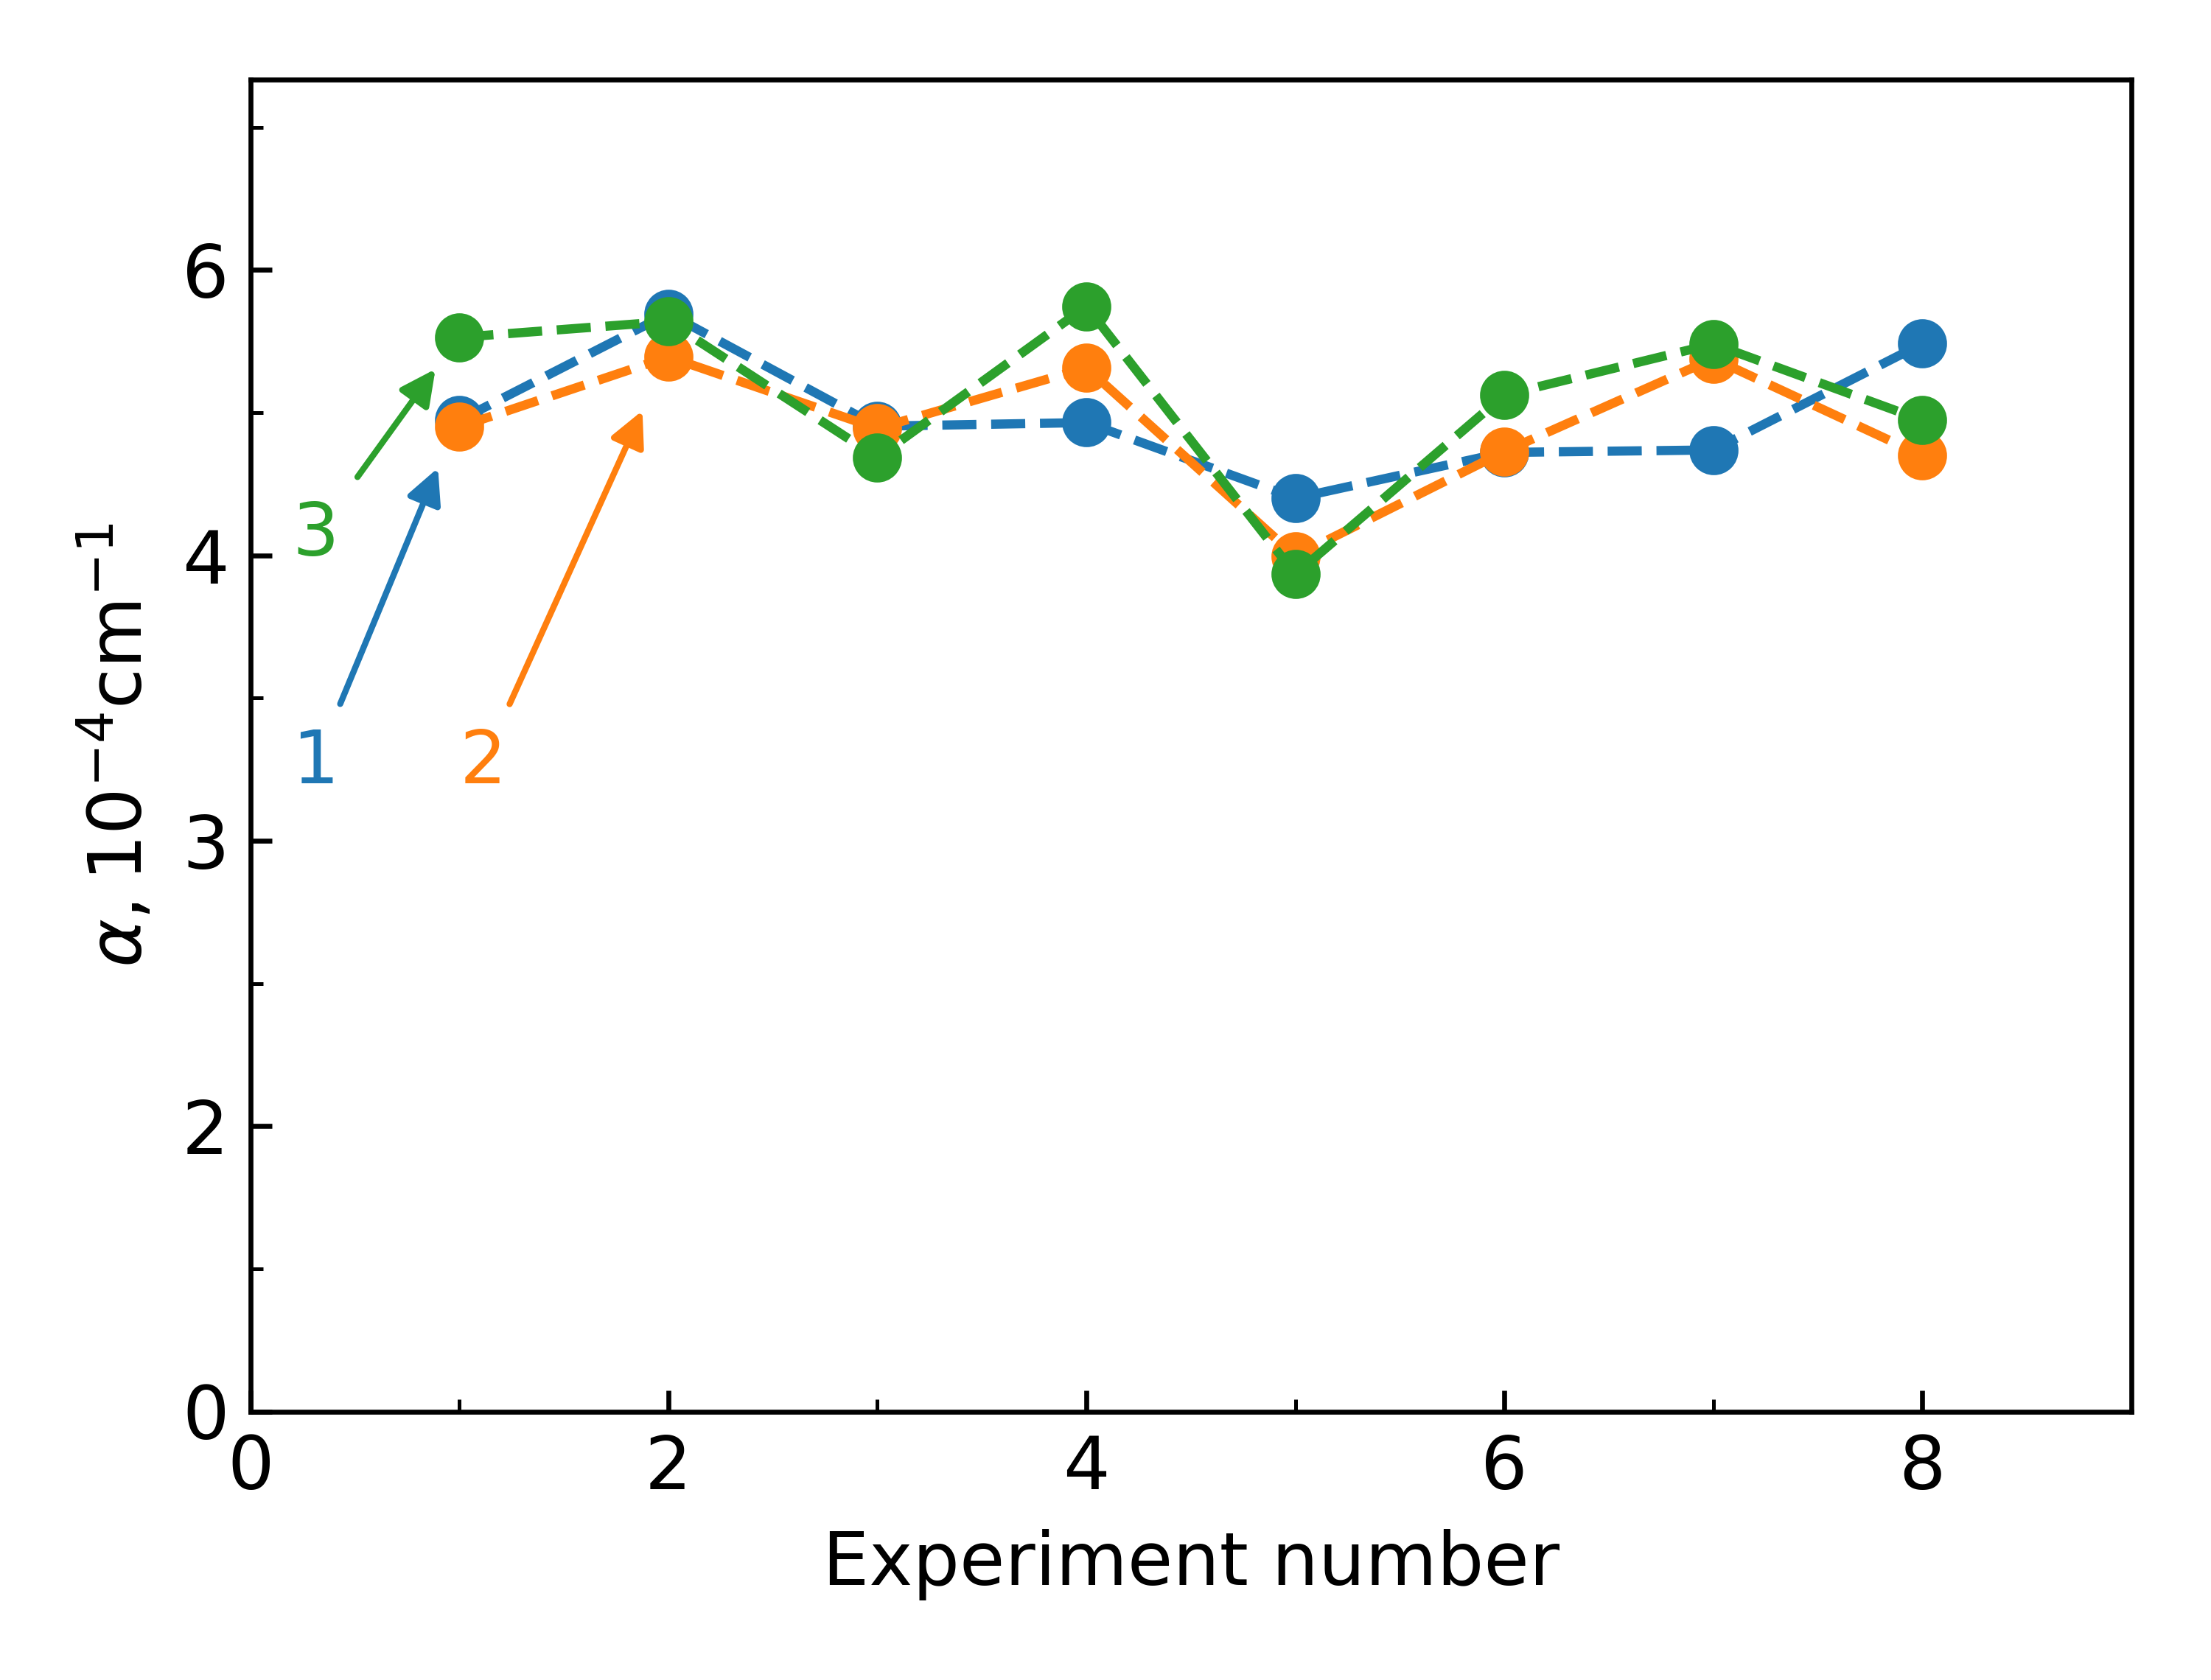
\includegraphics[width=\linewidth]{Dissertation/images/gradient/main_fourier_ambient_imponential}
		\end{column}

	\end{columns}	
	
	\vspace{-0.4cm}
	
	\begin{columns}		
		\begin{column}{0.4\textwidth}
			\centering
			{\scriptsize
			Схема установки:\\1 --- лазер (40~Вт, 1030~нм, диаметр пучка~---2~мм);\\2 --- измеритель резонансной частоты;3 --- компьютер;4 --- датчик температуры среды;\\5 --- измеритель мощности}
		\end{column}
		
		\begin{column}{0.6\textwidth}
			\centering
			{\footnotesize
			{\color{defcolor1}{1}}, {\color{defcolor2}{2}}, {\color{defcolor3}{3}}~--- {\color{defcolor1}{экспоненциальная}}, {\color{defcolor2}{импульсная}}, {\color{defcolor3}{градиентная}} методики\\
			Без поправок (слева), учёт ${dT_a}\left/{dt}\right.$ и $h$ (справа)
			}
						
		\end{column}
	\end{columns}	
	
	\vfill 
	\centering
	
	\begin{columns}
		\begin{column}{0.47\textwidth}
			\normalsize{
				\begin{tabular}{|c|c|}
					\hline
					& \makecell{Макс. различие\\между методиками, \%} \\
					\hline
					Без поправок & 25 \\
					\hline
					Учёт ${dT_a}\left/{dt}\right.$ & 20 \\
					\hline
					Учёт $h$ & 15 \\
					\hline
					Учёт ${dT_a}\left/{dt}\right.$ и $h$ & 10 \\
					\hline
				\end{tabular}
			}
		\end{column}
		\begin{column}{0.53\textwidth}
			\small
			Почему LBO:
			\begin{itemize}
				\setlength{\itemsep}{0.3em}
				\item Низкое оптическое поглощение \(\to\) слабый разогрев \(\to\) сильнее проявляется нестабильность \(T_a\);
				\item Большие размеры \((100\cdot50\cdot50~\text{мм}^3)\) \(\to\) низкая скорость теплоотдачи \(\to\) сильнее сказывается её нестабильность.
			\end{itemize}
		\end{column}
	\end{columns}
	
\end{frame}